\chapter{Open heavy-flavour production in proton-proton collisions}

\lettrine[lines=6,findent=0.pt]{O}{pen heavy-flavour} hadrons, composed of a heavy quark (charm or beauty) along with lighter quarks, are exclusively formed in high-momentum transfer processes due to the large masses of approximately 1.3 \gevcc and 4.2 \gevcc for charm and beauty quarks, respectively. As a result, they are created in the early stages of the collision, and their production cross-section in the partonic interaction can be evaluated perturbatively using QCD. Studying the production of open heavy-flavour hadrons in proton-proton (pp) collisions not only provides a crucial test of the perturbative QCD framework, but also allows to set constraints on models. Furthermore, measurements in proton-proton collisions, where the production of a deconfined medium is not expected due to the lower energy densities reached, are necessary ingredients for the study of heavy-ion collisions, where the properties of the QGP can be investigated. 

\section{Factorisation theorems}
The production of open heavy-flavour hadrons in proton-proton collisions can be described using the factorisation theorems~\cite{Collins:1989gx}, which allow for the separation of short-distance, perturbative behaviour from long-distance, non-perturbative phenomena. The total production cross-section can be expressed as
\begin{equation*}
    \sigma_{\text{pp}}^\mathrm{H} = \sum_\mathrm{a,b = g, q, \overline{q}} \int \de x_1 \de x_2 f_\mathrm{a/A}(x_1,\mu_F^2) f_\mathrm{b/B}(x_2,\mu_F^2) \hat{\sigma}_\mathrm{ab \rightarrow c} (x_1,x_2,\mu_F^2,\mu_R^2) D_\mathrm{c\rightarrow H}(z,\mu_F^2) \quad ,
\end{equation*}
i.e. the convolution of; i. the Parton Distribution Functions (PDFs) $f_\mathrm{a/A}(x_1,\mu_F^2)$ and $f_\mathrm{b/B}(x_2,\mu_F^2)$, describing the initial-state probability of finding a parton a in the proton A carrying a fraction $x_1$ of the proton's momentum, and a parton b in the proton B carrying a fraction $x_2$ of its momentum, respectively; ii. the hard partonic scattering cross-section $\hat{\sigma}_\mathrm{ab \rightarrow c} (x_1,x_2,\mu_F^2,\mu_R^2)$, defining the probability of producing the final state c from the collision of partons a and b; and iii. the Fragmentation Functions (FFs) $D_\mathrm{c\rightarrow H}(z,\mu_F^2)$, which describe the probability of a parton of type c fragmenting into a heavy-flavour hadron H with a momentum fraction $z$. While the PDFs and FFs are non-perturbative quantities, parametrised from experimental data and regarded as universal across different processes, the hard partonic scattering cross-section can be perturbatively calculated using QCD, albeit requiring specific evaluations for each process. Factorisation theorems have been widely used to describe the production of open heavy-flavour hadrons in proton-proton collisions, and have proven to be successful in modeling experimental data. Figure~\ref{fig:ppDmeson} shows the production cross-section of prompt and non-prompt $\mathrm{D^0}$-mesons in proton-proton collisions at $\sqrt{s} = 13$ TeV measured at midrapidity ($\lvert y\rvert<0.5$) as a function of the transverse momentum by the ALICE experiment~\cite{ALICE:2021mgk}, and compared to FONLL perturbative QCD calculations~\cite{Cacciari:1998it}. The term \emph{prompt} refers to charm-hadrons directly produced in the hadronisation of a charm quark or through the strong decay of a directly produced excited charm-hadron or charmonium state, while \emph{non-prompt} charm hadrons are produced in the decay of a hadron containing a beauty quark. The FONLL predictions are in good agreement with the non-prompt $\mathrm{D^0}$-meson production cross-section, whereas the prompt contribution lies at the upper edge of the theoretical uncertainty band, albeit being described within the uncertainties. Similar trends are observed in the production of other open heavy-flavour hadrons across different experimental facilities, such as the Tevatron, RHIC, and LHC.
\begin{figure}[htb]
    \centering
    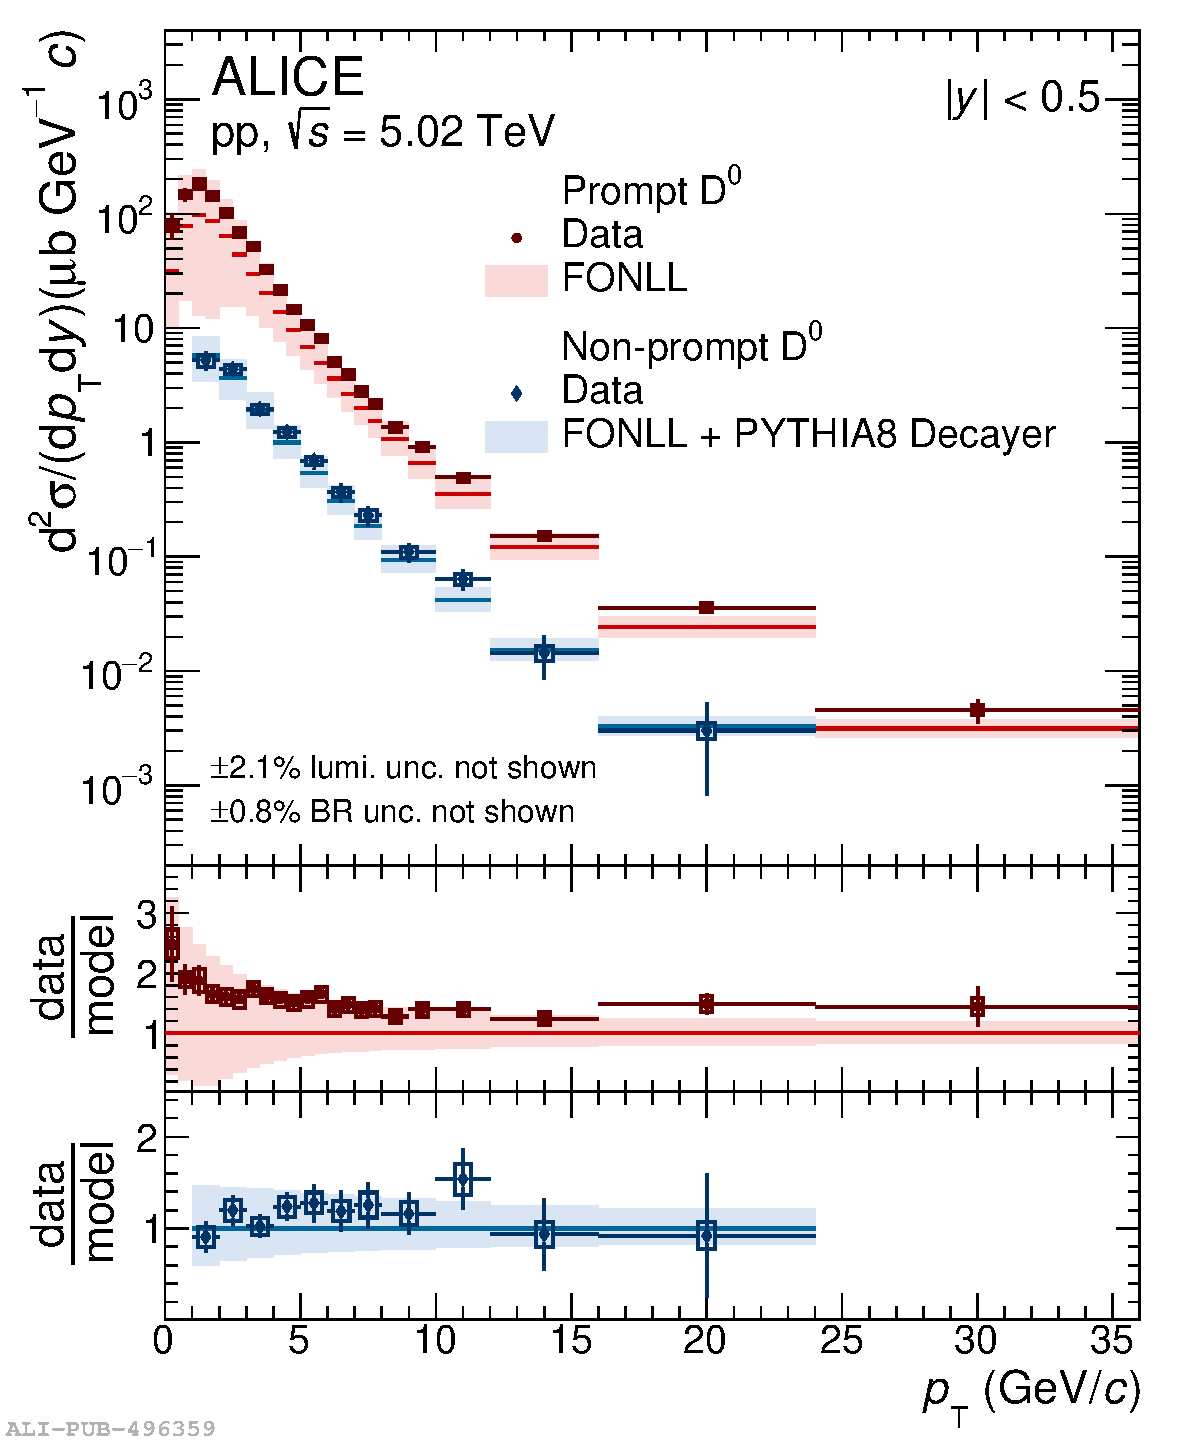
\includegraphics[width=0.6\linewidth]{Figures/Chapter 2/CrossSectionD0_Prompt_NonPrompt_pp5TeV_vsFONLL_Pythia8_BRnative_1.pdf}
    \caption{\pt-differential production cross-section of prompt and non-prompt $\mathrm{D^0}$-mesons~\cite{ALICE:2021mgk} compared to predictions obtained with FONLL calculations~\cite{Cacciari:1998it} combined with PYTHIA~8~\cite{Sjostrand:2014zea} for the $\mathrm{H_b \rightarrow D^0+X}$ decay kinematics.}
    \label{fig:ppDmeson}
\end{figure}

\subsection{Parton Distribution Functions}
\subsubsection{Deep inelastic scattering}
The PDFs are non-perturbative quantities describing the probability of finding a parton carrying a fraction $x$ of the proton's momentum in the initial state of a process. The first experimental evidence revealing the partonic structure of the proton emerged from deep inelastic scattering experiments carried out at the Stanford Linear Accelerator Center (SLAC) in the 1960s~\cite{Friedman:1972sy}, where an electron was scattered off a proton, and the transferred momentum $q$ was measured. The cross-section for deep inelastic scattering can be defined in terms of the Lorentz invariant variables $Q^2 = -q^2$ and $x = \frac{Q^2}{2P\cdot q}$, yielding
\begin{equation*}
    \frac{\de^2\sigma}{\de x \de Q^2} = \frac{4\pi\alpha^2}{xQ^4} \left[ \left(1-y\right)F_2(x,Q^2) - xy^2F_1(x,Q^2) \right]\quad ,
\end{equation*}
where $y=Q^2/(sx)$, $s = (P+p_\mathrm{e})^2$ denotes the centre-of-mass energy of the electron-proton system, and the structure functions $F_1(x,Q^2)$ and $F_2(x,Q^2)$ represent an extension of the form factors for elastic scattering.
The first measurements of high-energy inclusive inelastic scattering experiments were performed using a 20~GeV linear accelerator at SLAC, and showed that the structure functions $F_1(x,Q^2)$ and $F_2(x,Q^2)$ were independent of $Q^2$ at fixed $x$ within the studied $1<~Q^2~<~10$~\gevcc range. This was in contrast with the behavior observed for the proton elastic form factors, where a decrease of two orders of magnitude was observed within the same $Q^2$ interval. This independence of the structure functions from $Q^2$ in deep inelastic scatterings was predicted by Bjorken in 1968 for $Q^2 \rightarrow \infty$~\cite{Bjorken:1968dy}, and is known as \emph{Bjorken scaling}. A physical interpretation of this phenomenon arrived just one year later, in 1969, with Feynman's parton model~\cite{Feynman:1969ej}, which described the interaction in terms of elastic scattering of the probe off a point-like constituent (parton) within the proton. This model explains the scale-invariance property of the proton structure functions, as the scattering centres are assumed to be structure-less. In this picture, the Bjorken variable $x$ acquires a new interpretation as the fraction of the proton momentum carried by the struck parton. The parton model also offers a straightforward definition of the structure functions in terms of the parton distribution functions $f_\mathrm{a}(x)$:
\begin{equation*}
    F_2(x,Q^2) = \sum_\mathrm{a} e_\mathrm{a}^2 x f_\mathrm{a}(x)\quad ,
\end{equation*}
where the sum is over partons with electric charge $e_\mathrm{a}$, and $f_\mathrm{a}$ are unknown, but universal functions for a given hadron, describing the probability of finding a parton of type a with a fraction $x$ of the proton's momentum. 

To explore the spin properties of the partons, the structure functions $F_1$ and $F_2$ were studied at different centre-of-mass energies. By investigating the relationship between the two structure functions, it was established that the partons have spin 1/2, as the Callan-Gross relation~\cite{Callan:1969uq}, which holds true for point-like Dirac particles, was found to be satisfied:
\begin{equation*}
    F_2(x,Q^2) = 2x F_1(x,Q^2)\quad .
\end{equation*}

In the next years, it became clear that additional constituents within the proton carry momentum but lack electric or weak charge, as the so-called momentum sum rule was not saturated by the measured PDFs in electron and neutrino scatterings. This missing momentum was attributed to gluons, which were discovered in the 1970s and are the field quanta of the strong force.

\subsubsection{Bjorken scaling violation}
\begin{figure}[htb]
    \centering
    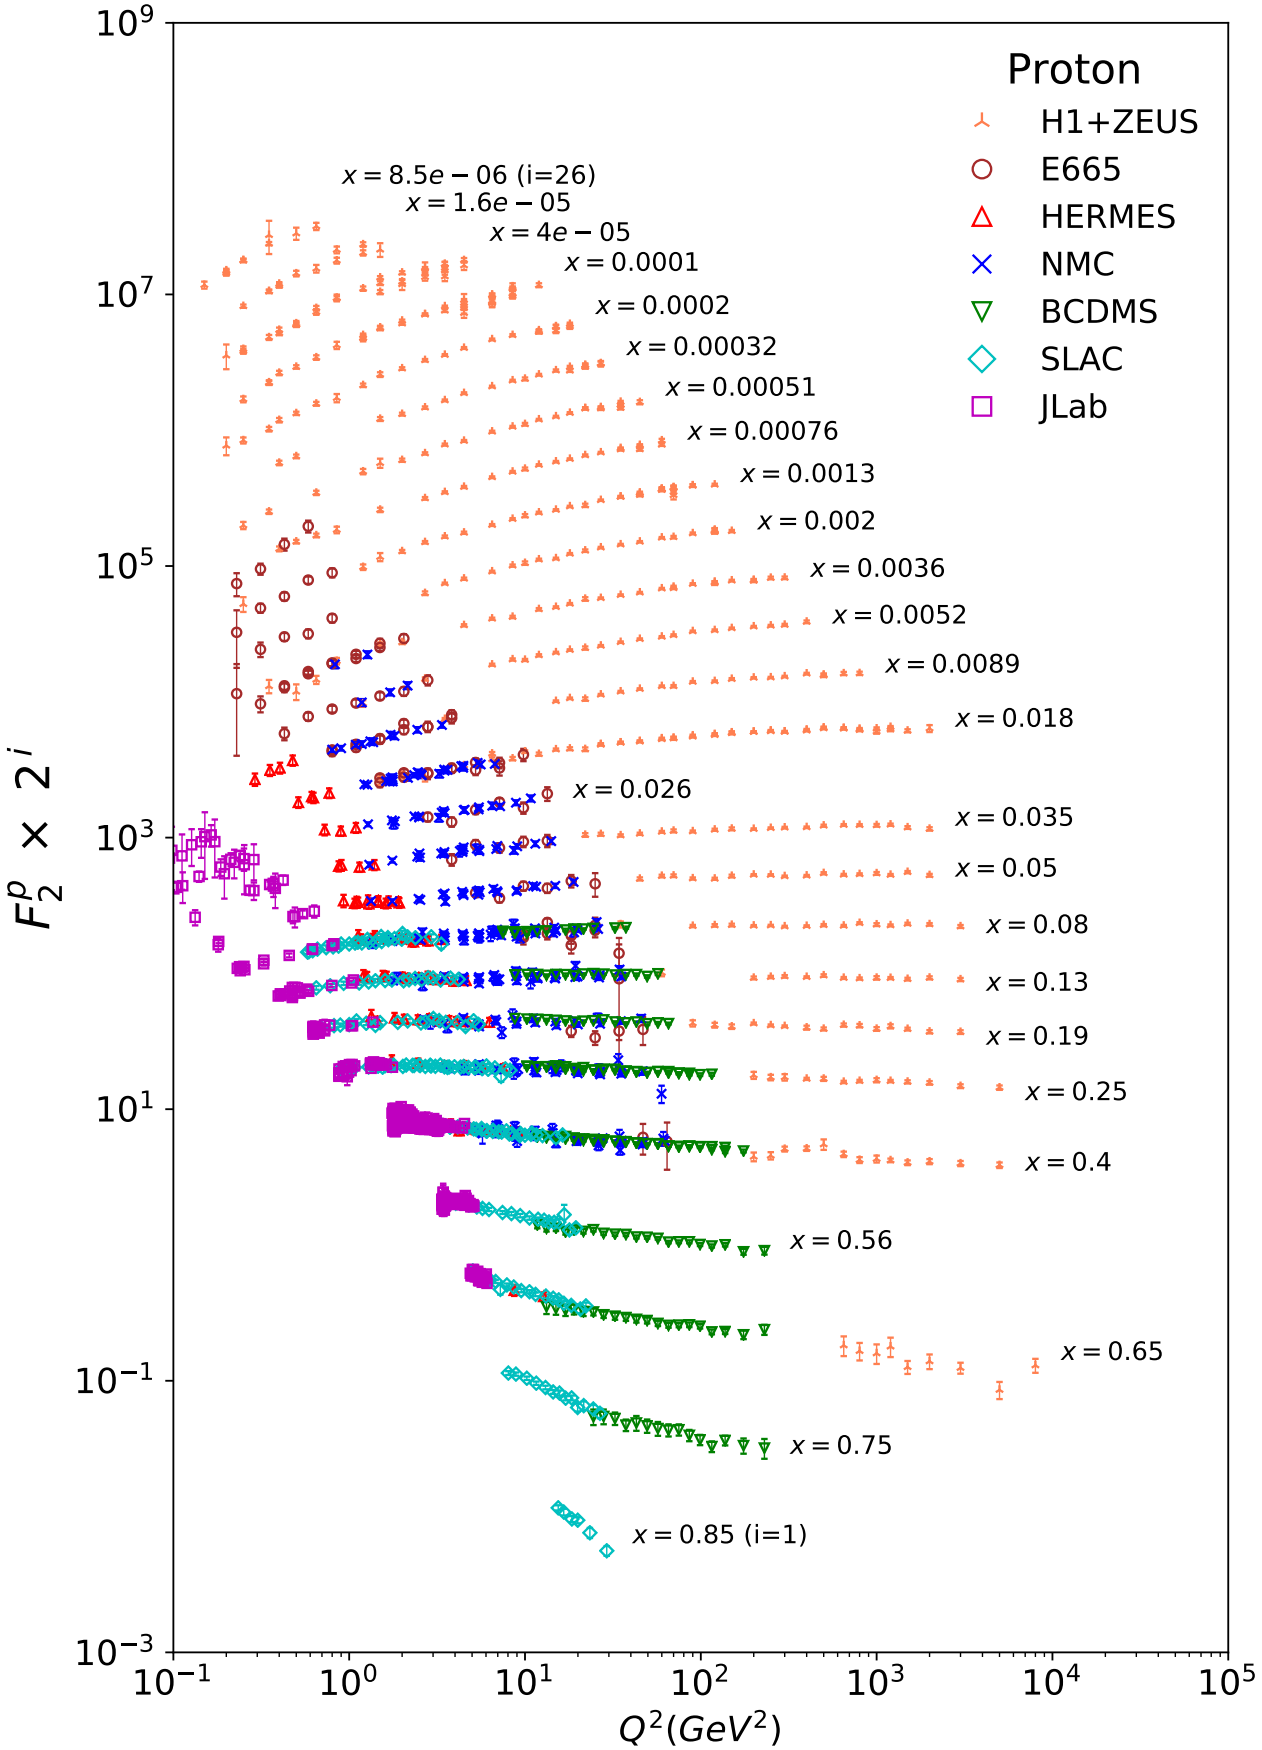
\includegraphics[width=0.6\linewidth]{Figures/Chapter 2/F2Results.png}
    \caption{The proton structure function $F^p_2$ measured in electromagnetic scattering of electrons and positrons on protons, and for electrons/positrons and muons on a fixed target~\cite{pdg}.}
    \label{fig:scaling_violation}
\end{figure}
By the late 1970s, measurements of the structure functions at larger $Q^2$ values taken at CERN and DESY revealed that Bjorken scaling was violated, i.e., the structure functions were not $Q^2$ independent. Figure~\ref{fig:scaling_violation} shows measurements of the proton structure functions $F_2(x,Q^2)$ as a function of $Q^2$ for various values of $x$ taken from different experiments~\cite{pdg}. It is clear from the plot that structure functions present an increasing trend as a function of $Q^2$ at low $x$, and a decreasing trend as a function of $Q^2$ at high $x$. 

The parton model fails to explain this behaviour, as it relies on the assumption that the transferred energy is sufficiently large to neglect the proton and its constituents' masses, as well as the interactions among partons. In particular, the partons' transverse momentum with respect to the proton momentum is neglected. The key to understanding Bjorken scaling violation comes from QCD and the realization that the parton's transverse momentum is not necessarily restricted to be small. A quark, for instance, can emit a gluon and acquire large transverse momentum $k_T$ with a probability proportional to $\als \de k_T/k_T^2$ at large $k_T$. The integral extends up to the kinematic limit $k_T\sim Q^2$, giving rise to contributions proportional to $\als\mathrm{log}Q^2$, which break scaling. The evolution of PDFs with $Q^2$ from a parametrisation at a given $Q^2_0$ can be perturbatively described using the Dokshitzer-Gribov-Lipatov-Altarelli-Parisi (DGLAP) evolution equations~\cite{Gribov:1972ri,Dokshitzer:1977sg,Altarelli:1977zs}, which require the introduction of a new arbitrary scale, at which the factorisation of the non-perturbative processes happens: the factorisation scale $\mu_F$. There exists a wide range of PDF parametrisations, such as the NNPDF~\cite{NNPDF:2021njg}, CTEQ~\cite{Dulat:2015mca}, and MMHT~\cite{Harland-Lang:2014zoa}, which are determined from global fits to a wide range of experimental data, including deep inelastic scattering, Drell-Yan, and jet production.
\subsection{Partonic cross-section}\label{sec:partonic_cross_section}
\begin{figure}[htb]
    \centering
    \begin{tikzpicture}
      \begin{feynman}
        \vertex (a);
        \vertex [above=1cm of a] (b) {q};
        \vertex[below=1cm of a] (c) {$\overline{\mathrm{q}}$};
        \vertex[right=1cm of a] (d);
        \vertex[right=0.7cm of d] (e);
        \vertex[right=1.3cm of e] (f);
        \vertex[right=0.7cm of f] (g);
        \vertex[right=1cm of g] (h);
        \vertex[above=1cm of h] (i) {Q};
        \vertex[below=1cm of h] (j) {$\overline{\mathrm{Q}}$};
        \diagram* {
            (b) -- [fermion] (d) -- [fermion] (c),
            (d) -- [gluon] (e),
            (e) -- [gluon,  in=90, out=90, looseness=1.7] (f) -- [gluon,  in=-90, out=-90, looseness=1.7] (e),
            (f) -- [gluon] (g),
            (j) -- [fermion] (g) -- [fermion] (i),
        };
      \end{feynman}
    \end{tikzpicture}\quad
    \begin{tikzpicture}
        \begin{feynman}
          \vertex (a);
          \vertex [above=1cm of a] (b) {q};
          \vertex[below=1cm of a] (c) {$\overline{\mathrm{q}}$};
          \vertex[right=1cm of a] (d);
          \vertex[right=0.7cm of d] (e);
          \vertex[right=1.3cm of e] (f);
          \vertex[right=0.7cm of f] (g);
          \vertex[right=1cm of g] (h);
          \vertex[above=1cm of h] (i) {Q};
          \vertex[below=1cm of h] (j) {$\overline{\mathrm{Q}}$};
          \diagram* {
              (b) -- [fermion] (d) -- [fermion] (c),
              (d) -- [gluon] (e),
              (e) -- [fermion,  in=90, out=90, looseness=1.7] (f) -- [fermion,  in=-90, out=-90, looseness=1.7] (e),
              (f) -- [gluon] (g),
              (j) -- [fermion] (g) -- [fermion] (i),
          };
        \end{feynman}
      \end{tikzpicture}

    \vspace*{0.5cm}
    \begin{tikzpicture}
        \begin{feynman}
          \vertex (a);
          \vertex [above=1cm of a] (b) {q};
          \vertex[below=1cm of a] (c) {$\overline{\mathrm{q}}$};
          \vertex[right=1cm of a] (d);
          \vertex[right=1cm of d] (e);
          \vertex[right=1cm of e] (f);
          \vertex[above=1cm of f] (g) {Q};
          \vertex[below=1cm of f] (h) {$\overline{\mathrm{Q}}$};
          \vertex[right=0.5cm of e] (i);
          \vertex[below=0.5cm of i] (j);
          \diagram* {
              (b) -- [fermion] (d) -- [fermion] (c),
              (d) -- [gluon] (e),
              (h) -- [fermion] (e) -- [fermion] (g),
              (j) -- [gluon, edge label = g] (f),

          };
        \end{feynman}
      \end{tikzpicture}\quad
      \begin{tikzpicture}
        \begin{feynman}
            \vertex (a);
            \vertex [above=1cm of a] (b) {q};
            \vertex[below=1cm of a] (c) {$\overline{\mathrm{q}}$};
            \vertex[right=1cm of a] (d);
            \vertex[right=1cm of d] (e);
            \vertex[right=1cm of e] (f) ;
            \vertex[above=1cm of f] (g) {Q};
            \vertex[below=1cm of f] (h) {$\overline{\mathrm{Q}}$};
            \vertex[right=0.5cm of e] (i);
            \vertex[below=0.5cm of i] (j);
          \diagram* {
              (b) -- [gluon] (d) -- [gluon] (c),
              (d) -- [gluon] (e),
              (h) -- [fermion] (e) -- [fermion] (g),
              (j) -- [gluon, edge label = g] (f),

          };
        \end{feynman}
      \end{tikzpicture}\quad
      \begin{tikzpicture}
        \begin{feynman}
          \vertex (a) {g};
          \vertex[above=0.25cm of a] (spacing) {$ $  }; 
          \vertex[right=1.25cm of a] (b);
          \vertex[right=1.45cm of b] (c) {q};
          \vertex[below=1.75cm of a] (d) {q};
          \vertex[right=1.25cm of d] (e);
          \vertex[right=0.75cm of e] (f);
          \vertex[right=1cm of f] (g);
          \vertex[above=0.3cm of g] (h) {Q};
          \vertex[below=0.3cm of g] (j) {$\overline{\mathrm{Q}}$};
          \diagram* {
                (a) -- [gluon] (b),
                (d) -- [fermion] (e) -- [fermion] (b) -- [fermion] (c),
                (e) -- [gluon] (f),
                (j) -- [fermion] (f) -- [fermion] (h),
          };
        \end{feynman}
      \end{tikzpicture}\quad
    \caption{Feynman diagrams contributing to the first order corrections of the heavy-flavour production cross-section calculations.}
    \label{fig:NLO_diagrams}
\end{figure}


Because of their large masses, heavy quarks can only be produced through hard-scattering processes, characterized by momentum transfers of the order of $Q^2 \geq 4m^2_\mathrm{b,c}$. In this regime, the strong coupling constant is significantly smaller than unity, allowing for the perturbative calculation of the heavy quark production cross-section from partonic scattering using QCD. While predictions at next-to-next-to-next-to-leading order (N$^3$LO) are available for certain processes, such as Higgs production~\cite{Anastasiou:2015vya, Anastasiou:2016cez}, the current state-of-the-art calculations for heavy quark production are at next-to-leading order (NLO) with all-order resummation to next-to-leading logarithmic (NLL) accuracy in the limit where the \pt of a heavy quark is much larger than its mass~\cite{Cacciari:1998it}. The contributions arising at the NLO include 1-loop virtual corrections to the Born process and real emission of a gluon or a quark-antiquark pair, and are depicted in Fig~\ref{fig:NLO_diagrams}.

\subsection{Fragmentation Functions}
\begin{sloppypar}
Quarks and gluons produced in hard-scattering processes ultimately give rise to colourless observable hadrons. The associated process, known as hadronisation, is non-perturbative and is described by the Fragmentation Functions (FFs) $D_\mathrm{c\rightarrow H}(z,\mu_F^2)$, which provide the probability of a parton of type c fragmenting into a hadron H with a momentum fraction $z$. FFs are typically determined from experimental data, usually by analyzing the final-state hadrons produced in electron-positron collisions where the initial momenta are well-known. These FFs are then applied in the evaluation of cross-sections in other colliding systems, assuming that the relevant hadronisation processes are “universal”, i.e., independent of the collision energy and system. Many FFs have been determined from global fits to data, such as the NNFF1.1h~\cite{Bertone:2018ecm}, DSS~\cite{deFlorian:2007aj}, and KKP~\cite{Kniehl:2000fe} parametrisations, and typically differ in the data sets used for the fit, the treatment of the data, and the functional form of the FFs. Similarly to PDFs, FFs also evolve with the energy scale of the interaction, and this evolution is described perturbatively by the DGLAP equations. 
\end{sloppypar}

\section{Hadronisation: from macroscopic to microscopic descriptions}
Despite being a very powerful tool for describing heavy-flavour hadron production, the factorisation theorem is not the only method used to describe the production of hadrons in high-energy collisions. Over the years, microscopic models have been developed to describe the hadronisation process and are typically implemented in Monte Carlo event generators. The standard approach for describing complex event topologies begins with a matrix-element calculation for the production of a few well-separated partons, followed by the application of a parton shower. 

The \emph{parton shower} provides an approximate perturbative treatment of QCD dynamics, which is then combined with a non-perturbative model for the hadronisation process at a certain infrared cut-off scale, typically taken to be of the order of 1~GeV. The basic idea of the parton shower relies on the Sudakov form factor~\cite{Sudakov:1954sw}, which expresses the probability of a parton not radiating another parton in a given phase space region. If a parton does radiate, the newly-produced parton becomes the source of a new cascade, continuing until the parton shower terminates at the hadronisation scale. At this point, partons are allowed to fragment into hadrons through hadronisation models. 

Although several hadronisation models have been developed, each implementing a different approach to the description of this non-perturbative process, a general approach is the hypothesis of local parton-hadron duality~\cite{Azimov:1984np}, which states that the flow of momentum and quantum numbers at the hadron level tends to follow the flow established at the parton level.

\subsection{Independent fragmentation}\label{sec:independent_fragmentation}
The description of the hadronisation process using FFs relies on the assumption of \emph{independent fragmentation}, i.e., the probability of a parton fragmenting into a hadron is considered independent of the other partons produced in the same collision. In the original scheme proposed by Field and Feynman~\cite{Field:1976ve}, the fragmenting quark combines with an antiquark from a $\mathrm{q\overline{q}}$ pair produced from the vacuum to create a meson with energy fraction $z$. The remaining quark, with energy fraction $(1-z)$, fragments in the same way, continuing until an energy cut-off is reached. The distribution of $z$ is the fragmentation function. The assumption of independent fragmentation is valid in the case of low-multiplicity \ee collision events, where the number of produced partons is small and no hadronic remnants are produced.
\subsection{String model}
\begin{figure}[htb]
    \centering
    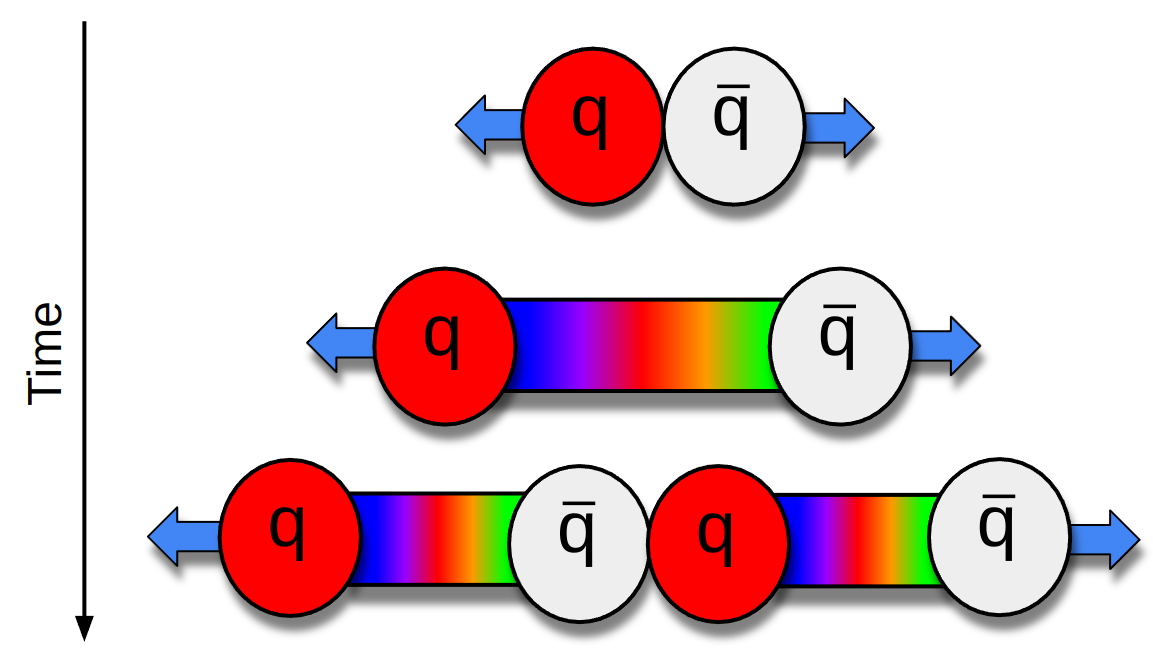
\includegraphics[width=0.7\linewidth]{Figures/Chapter 2/Lund.png}
    \caption{Schematic representation of the Lund string model hadronisation process.}
    \label{fig:Lund}
\end{figure}
The most widely used model for the description of the hadronisation process is the Lund string model~\cite{Andersson:1983ia}, employed in the PYTHIA event generator~\cite{Bierlich:2022pfr}. In this model, the strong force between quarks and gluons is modelled in terms of a colour string with energy given by the Cornell potential~\cite{Eichten:1974af},
\begin{equation*}
    V(r) = -\frac{A(r)}{r} + \kappa r\quad .
\end{equation*}
Since the linear term is dominant, the Cornell potential is typically approximated as $V(r) = \kappa r$, with $\kappa\sim1$~\gev/fm. This implies that a constant force is exerted between the quarks, leading to a linear increase in the potential energy with the distance between the quarks. When back-to-back quarks are produced in a hard-scattering process, they move apart, causing the string to stretch and accumulate energy. When the energy stored in the string becomes large enough, it becomes energetically convenient to materialise a quark-antiquark pair from the colour flux tube, making the string break. The probability of string breaking is given by
\begin{equation*}
    P \propto exp\left(-\frac{\pi m_\mathrm{T,q}^2}{\kappa}\right) = exp\left(-\frac{\pi m_\mathrm{q}^2}{\kappa}\right) exp\left(-\frac{\pi p_\mathrm{T,q}^2}{\kappa}\right)\quad .
\end{equation*}
The mass dependence of this equation leads to a gaussian suppression factor that limits the probability for the colour field to produce quark-antiquark pairs for heavier flavours. The $s\overline{s}$ and $c\overline{c}$ pair production probability can be estimated with respect to that for $u\overline{u}$ and $d\overline{d}$ pairs~\cite{Ferreres-Sole:2018vgo}, yielding
\begin{equation*}
    u : d : s : c \sim 1 : 1 : 1/3 : 10^{-11}\quad .
\end{equation*}
The soft production of $c\overline{c}$ results significantly suppressed, by a factor of $10^{-11}$, compared to $u\overline{u}$ pairs. Such quarks are therefore almost exclusively produced in hard-scattering processes, quantitatively confirming the qualitative discussion in Sec.~\ref{sec:partonic_cross_section} on the feasibility of using perturbative QCD to describe the production of heavy-flavour quarks.

\subsubsection{Non-independent fragmentation and multiple parton interactions}
The fragmentation model described above shares many similarities with the independent fragmentation model discussed in Sec.~\ref{sec:independent_fragmentation}, with the main difference being the pictorial description of interactions with a colour string connecting the quarks. However, the gluon radiation has been neglected until now. A significant difference emerges once the gluon bremstrahlung is considered~\cite{Sjostrand:1984ic}. 

In this framework, gluons are represented as carrying both a colour and an anticolour charge. Therefore, in a three-parton system ($\mathrm{q\overline{q}g}$), the quark is colour-connected to the anticolour index of the gluon, and the colour index of the gluon is connected to the antiquark. The interaction between the quark-antiquark pair is suppressed by a factor 1/$\mathrm{N_c}$, where $\mathrm{N_c}$ is the number of colours, and can be neglected in a leading-colour approximation ($\mathrm{N_c} \rightarrow\infty$). The presence of the gluon produces a corner, or “kink”, on the string. The Lorentz boost of a string causes the hadrons it forms through its breaking to go preferentially in the direction of its motion. Most hadrons that the q-g string segment produces will go between the quark and the gluon, while hadrons from the $\mathrm{\overline{q}\text{-}g}$ will go between the gluon and the antiquark. Only very few hadrons will go between the quark and the antiquark. This behaviour leads to an angular distribution of hadrons in \ee three-jet final states which differs from that predicted by independent fragmentation and is found to be in better agreement with experimental results. In the leading-colour approximation partonic final states, each quark is colour-connected to a single other parton in the event. Since gluons carry both a colour and an anticolour charge, they are connected to two other partons. With this aprroximation, the Lund model provides a good description of measurements in \ee collisions, where a parton-rich environment is not produced. However, recent results on the production of heavy-flavour baryons in proton-proton and proton-lead collisions at the LHC~\cite{ALICE:2022exq,ALICE:2024ozd} show that a description of the hadronisation process based on independent fragmentation is not sufficient to describe the data, as it significantly underestimates the baryon production.

In hadronic collisions, one must consider that for a comprehensive description of a given process, a description of coloured initial-state partons and their associated remnants should be taken into account, as they hadronize and may potentially interact with each other. Furthermore, new insights on the underlying event and soft-physics processes occurring in a hadronic collision suggest that they are dominated by Multiple Parton Interactions (MPI), where two or more distinct hard-parton interactions occur in a single hadron-hadron collision. Phase-space overlaps among the partons produced in the MPIs become more likely as the number of partons in the collision increases, and their non-independent hadronisation should be considered for a more complete description of the process. 

New models based on colour-reconnection beyond the leading-colour approximation~\cite{Christiansen:2015yqa} have been developed, where the leading-colour connections produced in the partonic showers are rearranged to form new subleading topologies that would have been present in a full-colour treatment. In addition, new colour junctions allow for an enhanced production of baryons, to account for the observed enhancement in the production of baryons in proton-proton and proton-lead collisions.

\subsection{Cluster model}
A different approach to the description of the hadronisation process is the cluster model~\cite{Webber:1983if}, which is implemented in the HERWIG event generator~\cite{Bahr:2008pv}. It is based on the \emph{preconfinement} of colour~\cite{Amati:1979fg}, which arises from the observation that by following the colour structure of the parton shower and studying the colour-singlet pairs of colour-connected quark-antiquark states, one finds that they tend to end up close in phase space. This suggests that quarks and gluons produced in this evolution become organized in clusters of colour singlets with finite masses, i.e., the mass distribution of these clusters is independent of the hard scattering process and its centre-of-mass energy. The confinement can then convert these singlets of small mass into hadrons. 

The first step of the cluster hadronization model is to non-perturbatively split the gluons left at the end of the parton shower into quark-antiquark pairs. Each gluon is allowed to decay into any of the accessible quark flavours with a probability given by the available phase space for the decay. 

Then, the hadronisation process takes place. The key idea is that because the cluster mass spectrum is both universal and steepling falling at high masses, the clusters can be regarded as highly excited hadron resonances and decayed, according to phase space, into the observed hadrons. Before the actual cluster decays, a few heavier clusters are split into lighter clusters before they decay (\emph{cluster fission}), for a more reasonable agreement with the experimental results. A cluster is split into two clusters if the mass, $M$, is such that
\begin{equation*}
    M^{\mathrm{Cl_{pow}}} \geq \mathrm{Cl_{max} {}^{Cl_{pow}}} + (m_1+m_2)^{\mathrm{Cl_{pow}}}\quad ,
\end{equation*}
where $\mathrm{Cl_{max}}$ and $\mathrm{Cl_{pow}}$ are parameters of the model, and $m_{1,2}$ are the masses of the constituent partons of the cluster. For clusters that need to be split, a $\mathrm{q\overline{q}}$ pair is produced from the vacuum. Only up, down and strange quarks are chosen with probabilities given by other model parameters. Once a $\mathrm{q, \overline{q}}$ pair is produced, the cluster is decayed into two new clusters with one of the original partons in each cluster. 

Finally, the cluster is decayed into a pair of hadrons. For a cluster of a given flavour ($\mathrm{q_1, \overline{q}_2}$), a quark-antiquark or diquark-antidiquark pair ($\mathrm{q\overline{q}}$) is extracted from the vacuum and a pair of hadrons with flavours ($\mathrm{q_1, \overline{q}}$) and ($\mathrm{q, \overline{q}_2}$) is formed. The hadrons are selected from all the possible hadrons with the appropriate flavour based on the available phase space, spin and flavour of the hadrons. As a consequence, heavier hadrons are suppressed, leading to a natural description of the baryon and strangeness suppression. The cluster model was found to describe data reasonably well, with far fewer parameters than the string model~\cite{Seymour:2013ega}.

\section{Coalescence model}
\begin{figure}[htb]
    \centering
    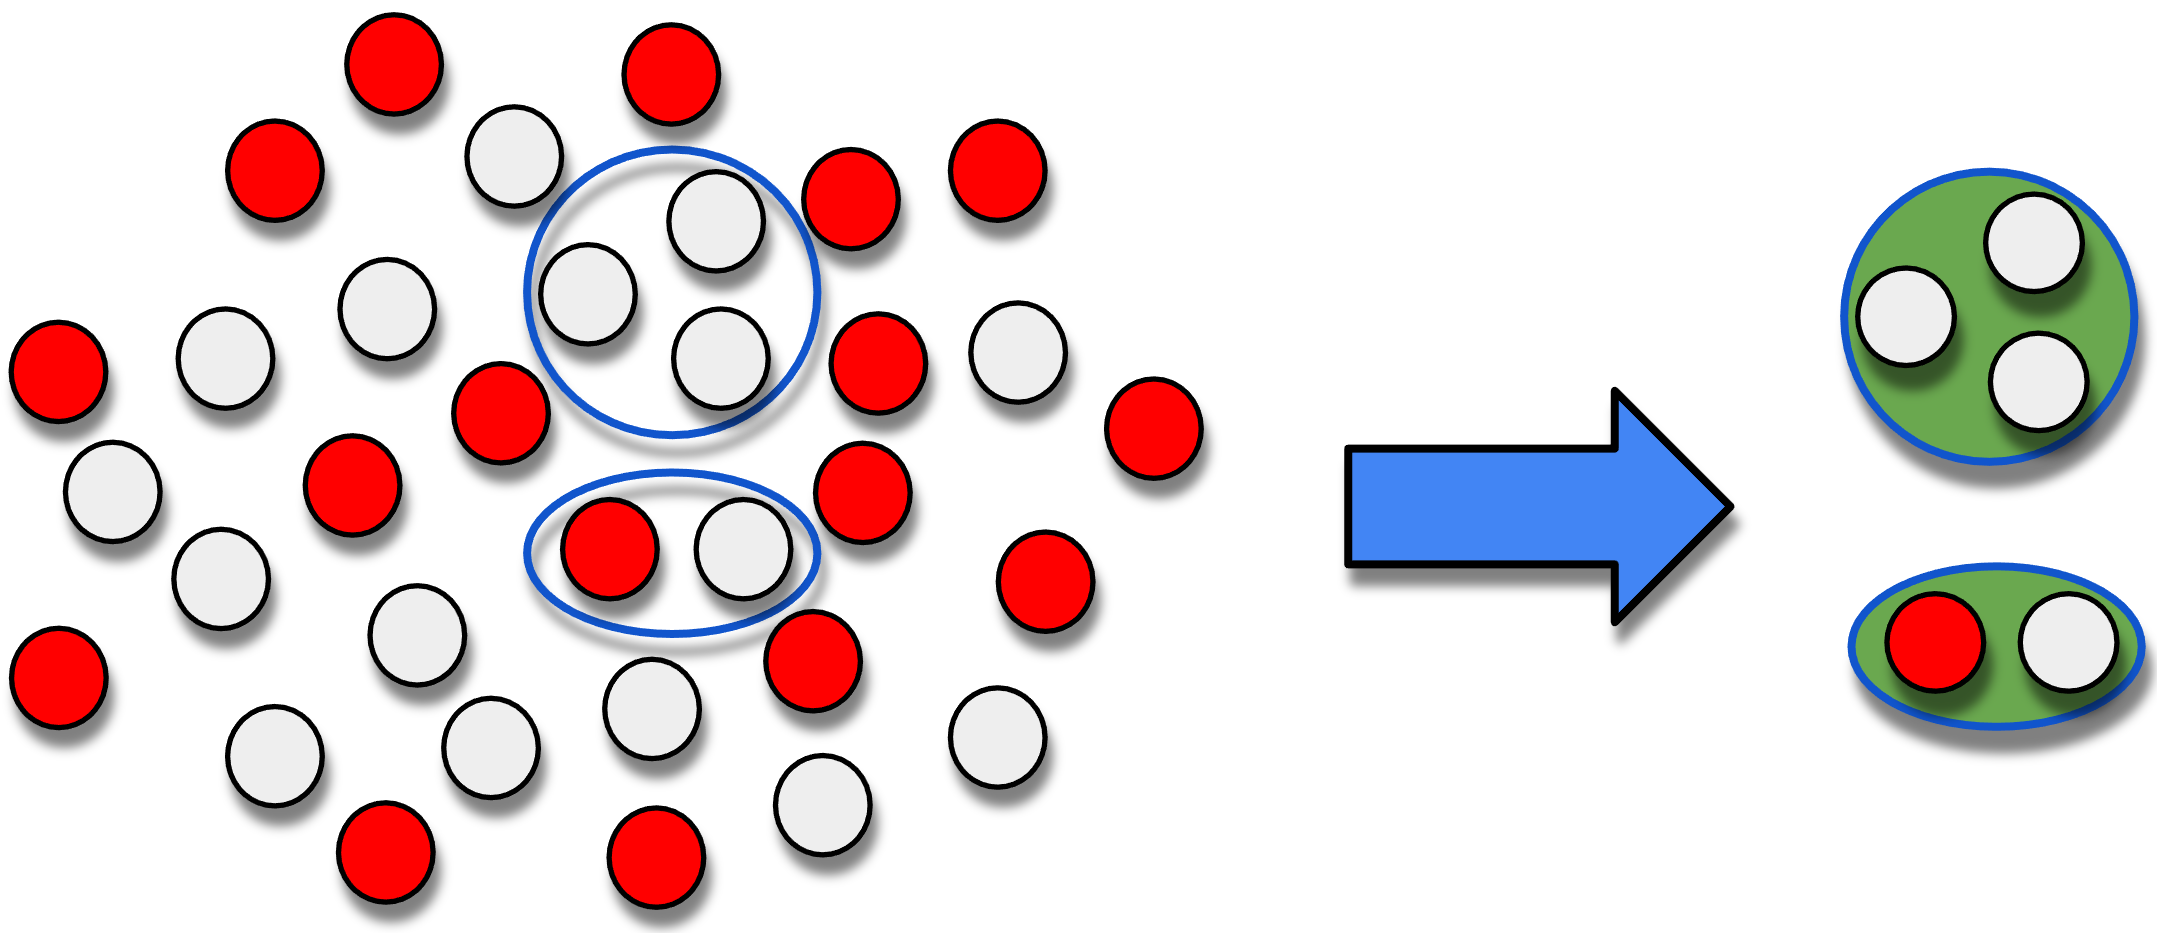
\includegraphics[width=0.7\linewidth]{Figures/Chapter 2/Coalescence.png}
    \caption{Representation of hadron production via recombination.}
\end{figure}

As outlined in Sec.~\ref{sec:high_pt}, the hadronisation process can be modified in the presence of a strongly-interacting deconfined medium. A novel mechanism for the production of hadrons, the recombination (also called coalescence), can take place in a thermalised system such as the QGP. When recombination occurs, low \pt partons close in the velocity-space phase space can bind together to form a higher-\pt hadron. This could lead to a depletion of the low-\pt hadron yield, and an enhancement of the intermediate-\pt hadron yield. This process modifies the production of hadrons in heavy-ion collisions, where the large amount of produced partons increases the probability of recombination. For this reason, the description of fragmentation functions derived from \ee collisions, where coalescence does not play a role, becomes inadequate. 

Only models implementing the coalescence mechanism can effectively describe the production of hadrons in heavy-ion collisions. Intriguingly, models implementing recombination that successfully describe the production of hadrons in these collisions, fail in doing so when this process is de-activated, as shown in Fig.~\ref{fig:D_recombination}. 

\begin{figure}[htb]
  \centering
  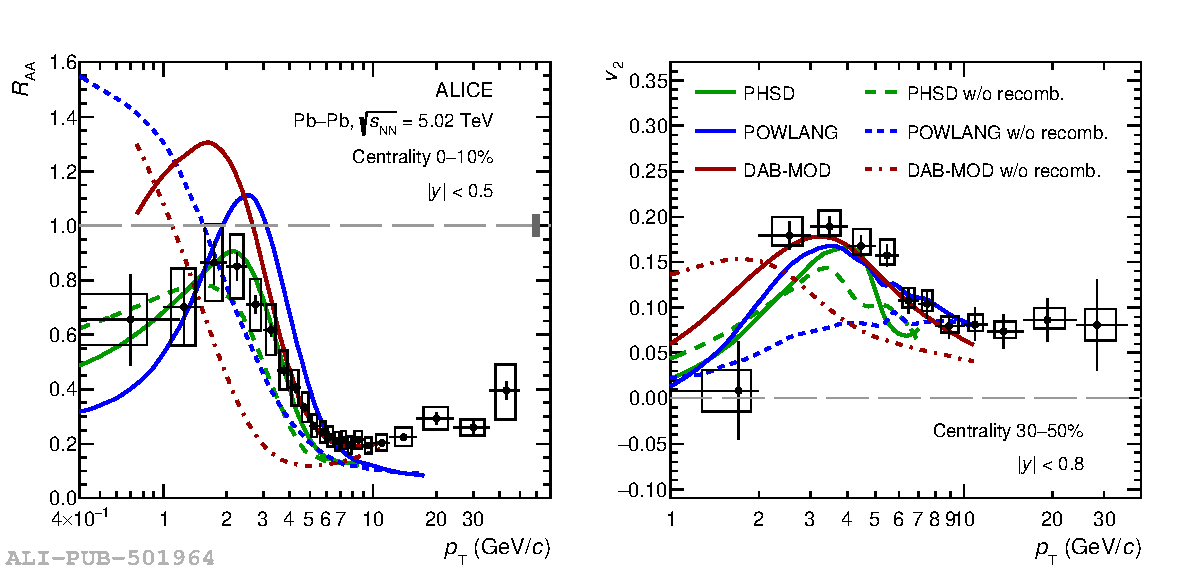
\includegraphics[width=\linewidth]{Figures/Chapter 2/D_Raa010_V23050_FragCoal_3models_1.pdf}
  \caption{Prompt D-meson $R_\mathrm{AA}$ in the 0--10\% centrality class (left panel) and $v_2$ in the 30--50\% centrality class (right panel) compared with predictions obtained with and without including hadronisation via recombination. Taken from~\cite{ALICE:2021rxa}.}
  \label{fig:D_recombination}
\end{figure}

New experimental measurements in pp and p--Pb collisions at the LHC~\cite{ALICE:2016fzo,ALICE:2020wla,ALICE:2024ozd,ALICE:2020wfu,ALICE:2021bli,CMS:2015fgy} provided a wealth of results suggesting that certain phenomena that are observed in nuclear collisions, such as strangeness enhancement and flow, may also occur in smaller collision systems. These effects are typically related to the presence of collective behaviours, thus raising the question of whether the coalescence hadronisation mechanism of coalescence could also play a role in small collision systems. A hint that this could be the case comes from the observation that the production of charm baryons in pp and p--Pb collisions~\cite{ALICE:2022exq,ALICE:2024ozd} is significantly larger than expected from models based on a independent fragmentation tuned on \ee collisions. 

Various models have been developed in order to describe the observed charm-baryon enhancement in proton-proton and proton-lead collisions with the assumption of a recombination mechanism. These include the Quark (re-)Combination Mechanism~\cite{Song:2018tpv} model, where coalescence between a charm quark and equal-velocity light quarks from fragmentation takes place, and thermal weights are applied to account for relative production of scalar and vector mesons. In addition, the assumption of equilibrium allows for a macroscopic description of the system using a hydrodynamic appoach: the Catania coalescence model~\cite{Minissale:2020bif} describes a thermalised system of $u$, $d$, $s$ quarks, and gluons, where the charm quark can hadronise via either fragmentation or coalescence with light quarks from the bulk, while, the POWLANG model~\cite{Beraudo:2023nlq} predicts the formation of a small, deconfined and expanding fireball in proton-proton collisions, where charm quarks are subject to rescattering and hadronization, and can recombine with light quarks as in heavy-ion collisions. Each of these models provides a different hadronization mechanism in proton-proton collisions compared to \ee ones, and independent hadronization is no longer assumed. 

\subsection{Core-corona model}
Core-corona models~\cite{Werner:2007bf} offer an intermediate approach between the two presented above. In these models, the fireball is divided into a hihg-density core part, treated with hydrodynamics and heavy-ion freeze-out models, and a corona part, described using the Lund string model. This framework is based on the assumption that small QGP droplets may be produced once the density is high enough. The EPOS Monte Carlo event generator~\cite{Porteboeuf:2008fgf} implements such a picture, and provides a very competitive description of data.

\subsection{Statistical hadronisation model}
The last model presented in this section exploits the idea of a thermalised system, which is by definition in thermal equilibrium. A macroscopic approach to hadronisation, based on a statistical model, can be used to describe the charm-hadron production in hadronic collisions. The principles of thermodynamics can be applied to the hadronisation process, where the hadron yields are determined by the hadron's mass and the temperature and baryon chemical potential of the system. As described in Sec.~\ref{subsec:SHM}, this approach has been successfully adopted to describe the light and strange hadron production in heavy-ion collisions and in smaller systems. However, the description of heavy-flavour hadron production and the baryon enhancement in this framework requires the inclusion of a strong feed-down from an augmented set of excited charm- or beauty-baryon states, not included in the PDG~\cite{pdg}. Recent model developments~\cite{He:2019tik,He:2022tod} have extended the Statistical Hadronisation Model (SHM) to include a set of 18 $\mathrm{\Lambda_c}$'s, 42 $\mathrm{\Sigma_c}$'s, 62 $\mathrm{\Xi_c}$'s, and 34 $\mathrm{\Omega_c}$'s up to a mass of 3.5~\gev, predicted by the Relativistic Quark Model~\cite{Ebert:2011kk}. Such model provides a good description of the measured $\mathrm{\Lambda_c/D^0}$ production yield ratio and the \pt spectra of D mesons and $\mathrm{\Lambda_c}$ at midrapidity.

\subsection{Baryon enhancement: \texorpdfstring{\boldmath$\mathrm{\Lambda_c/D^0}$}{Lc/D0} ratio}
\begin{figure}[htb]
    \centering
    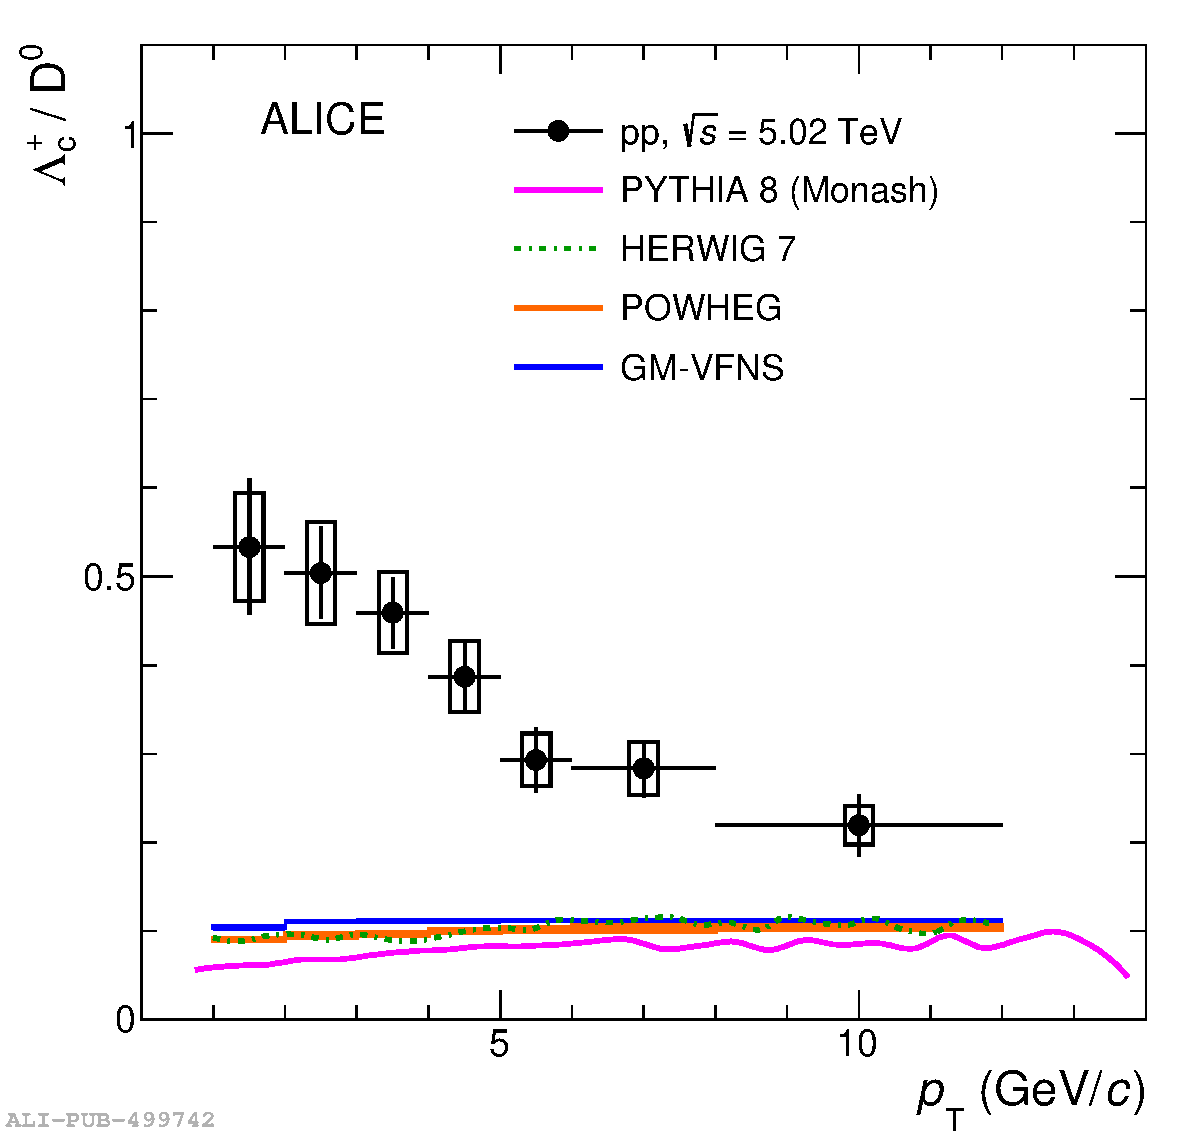
\includegraphics[width=0.48\linewidth]{Figures/Chapter 2/LcD_models_withFFModels_ropes_2.pdf}
    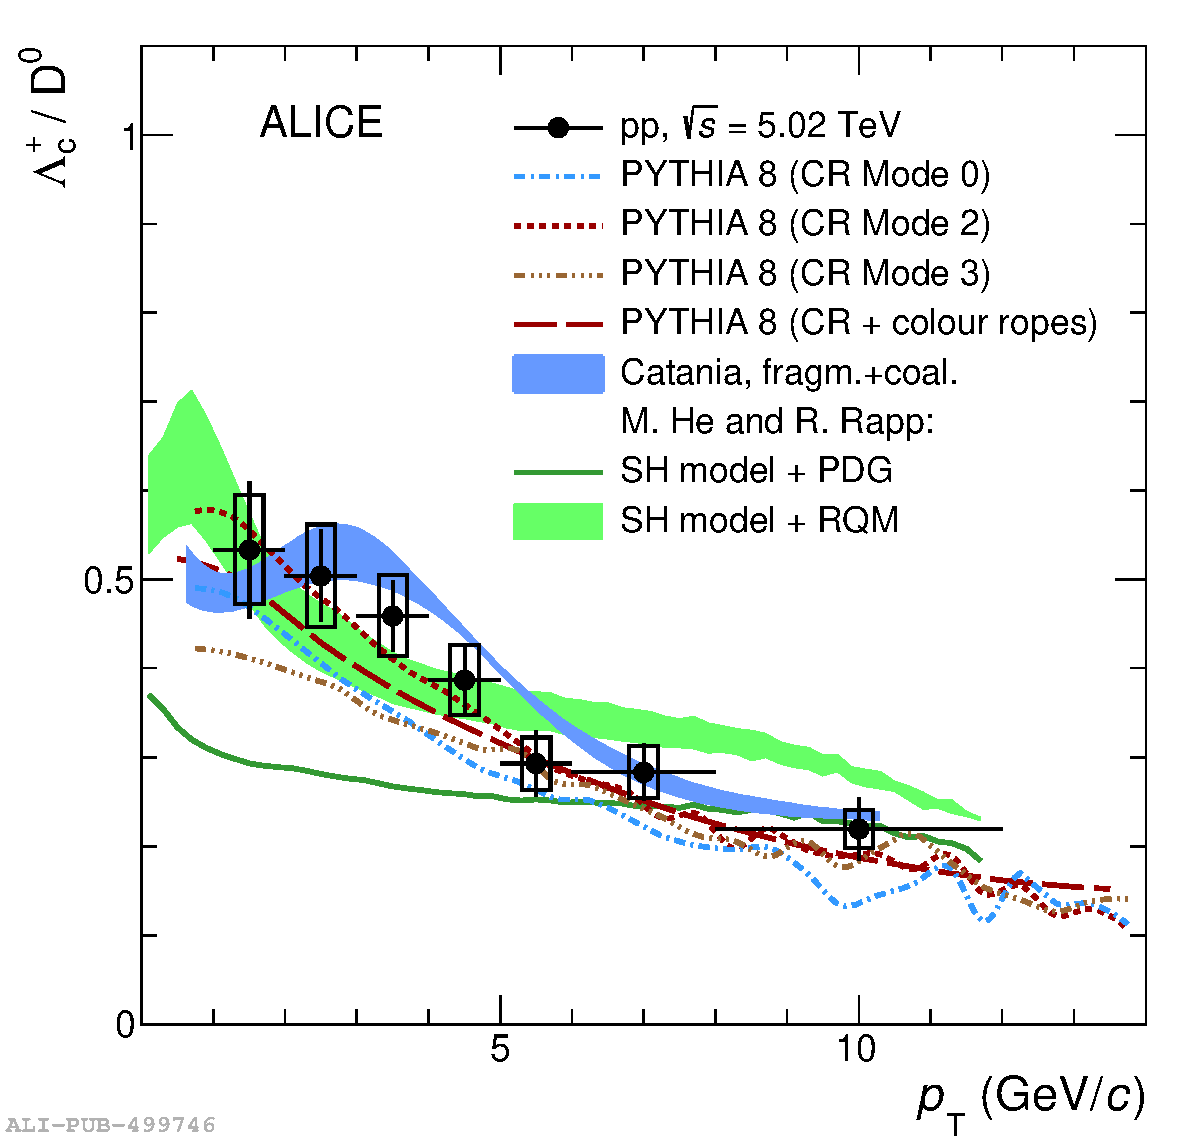
\includegraphics[width=0.48\linewidth]{Figures/Chapter 2/LcD_models_withModifiedModels_ropes_coal_2.pdf}
    \caption{$\mathrm{\Lambda_c/D^0}$ production yield ratio as measured at $\sqrt{s} = 13$~TeV by the ALICE Collaboration as a function of \pt, compared to theoretical predictions. Taken from~\cite{ALICE:2020wla}.}
    \label{fig:Lambda_c_D0}
\end{figure}
The hadronisation process can be experimentally studied through the measurement of production yield ratios of hadrons. Since the initial state of the collision and the charm production cross section is the same for all charm hadrons, the measurement of the production yield ratio of different charm hadrons can be expressed, using the factorisation theorem, as the ratio of the fragmentation functions of the hadrons, which describe the hadronisation process. Fig.~\ref{fig:Lambda_c_D0} shows the $\mathrm{\Lambda_c/D^0}$ production yield baryon-to-meson ratio measured at $\sqrt{s} = 13$~TeV by the ALICE Collaboration as a function of \pt, compared to theoretical predictions. 

In the left panel, the data are compared to i. PYTHIA~8 with Monash tune~\cite{Skands:2014pea}; ii. HERWIG~7~\cite{Bellm:2015jjp}; iii. POWHEG~\cite{Frixione:2007nw} NLO pQCD calculations, matched with PYTHIA~6 to generate the parton shower; iv. General-Mass Variable-Flavour-Number scheme (GM-VFNS~\cite{Kniehl:2005mk}) NLO pQCD calculation with next-to-leading-log resummation. All these models implement fragmentation processes tuned on results of charm production measurements is \ee collisions, and predict an almost \pt-idependent $\mathrm{\Lambda_c/D^0}$ ratio of around 0.1, significantly underestimating the measured values by a factor of about 7 at low \pt.

In the right panel, the measurements are compared to models that include mechanisms to enhance baryon production. They include i. PYTHIA~8 simulations with colour-reconnection beyond the leading-colour approximation~\cite{Christiansen:2015yqa} (three colour reconnection modes (0,2,3), which apply different constraints on the allowed reconnection are considered); ii. PYTHIA~8 with colour-reconnection plus rope hadronisation~\cite{Bierlich:2014xba} where colour charges can act coherently to form a rope, increasing the effective string tension; iii. Catania coalescence model~\cite{Minissale:2020bif}, where a QGP is formed in pp collisions and hadronisation occurs through both recombination and fragmentation; iv. SHM~\cite{Braun-Munzinger:2003pwq} where the underlying charm baryon spectrum is either taken from the PDG~\cite{pdg}, or augmented to include additional excited baryon states, which have not yet been observed but are predicted by the RQM~\cite{Ebert:2011kk}. These models are capable of describing both the magnitude and the \pt dependence of the $\mathrm{\Lambda_c/D^0}$ ratio, suggesting that the hadronisation process in proton-proton collisions might differ from that in \ee collisions.

The influence of the surrounding environment in the hadronisation of the charm quark could also potentially explain the observed strangeness enhancement in proton-proton collisions when compared to \ee collisions. Enhanced production of charm-strange hadrons may result from the coexistence of numerous strange quarks (which could be thermally produced in an environment with $T \gg m_\mathrm{s}$) within the same region as the charm quark, thereby increasing the probability of recombination between them. This phenomenon can be studied through the measurement of the production yield ratio of charm-strange hadrons to non-strange charm hadrons, such as the $\mathrm{D_s^+}$-meson to $\mathrm{D^+}$-meson ratio, which constitutes the primary focus of this Thesis.